\section{The Gaussian}
\label{section:gaussian}

Given a sufficiently large numerical population in many cases this population's distribution of values will converge toward the the same shape, the Gaussian distribution, also known as the Normal Distribution or bell curve. Common examples of this are a human population's height, weight and blood pressure \cite{modern_statistics}. This distribution is useful in image processing and computer vision because it can be used to predict the distribution of numerical measures of an image, like the distribution of colours in an image. \emph{The Central Limit Theorem}, the Normal Distribution's accompanying theorem, states that even when an individual random variable doesn't converge to the normal distribution, sums and averages of the variable will converge to some approximation of the distribution \cite{modern_statistics}. 

\textbf{The Gaussian distribution function} models the shape of the Gaussian distribution and is described by the equation \ref{eq:gauss}. A continuous random variable X is said to be distributed normally if it's probability density function is modelled by equation \ref{eq:gauss} if $-\infty < \mu < \infty$ and $0 < \sigma$.


\begin{equation}
  \mathcal{N}(x|\mu,\sigma) = \frac{A}{\sqrt{2\pi}\sigma}e^{-\frac{1}{2}(\frac{x-\mu}{\sigma})^2}
\label{eq:gauss}
\end{equation}

The variables $\mu$, $A$ and $\sigma$ represent the mean, amplitude and standard deviation of the distribution respectively. The mean, $\mu$, is the average value of all samples, it is also the distributions middle value, median, and most common value, mode. Half of all samples have a value greater than the mean, and half of all values have a values less than the mean. The amplitude, $A$, is the value of the \emph{distribution} at the mean, it is the largest value of the distribution because the mean is the value with the greatest \emph{likelihood}, where likelihood is the probability that given a distribution of data $x$, a piece of data $x_i$ has a specific value. The standard deviation, $\sigma$ is a measure of the distributions spread and is calculated as in equation \ref{eq:standard_deviation}, note that $N$ is the number of samples in a distribution. Figure \ref{fig:gauss} shows a one-dimensional Gaussian distribution and indicates where the mean, amplitude and standard deviation are.

\begin{equation}
  \sigma = \sqrt{\frac{1}{N}\sum_{i=1}^{N}(x_i - \mu)^2}
  \label{eq:standard_deviation}
\end{equation}

The Gaussian Distribution of a D-dimensional vector $\boldsymbol{x}$ is described by equation \ref{eq:gauss_multi}, where \textbf{$\mu$} is D-dimensional mean vector, \textbf{$\Sigma$} is D x D covariance matrix and $\|\boldsymbol{\Sigma}\|$ is the determinant of \textbf{$\Sigma$} \cite{patterns_machine_learning}. Covariance is a measure of two variables joint variability, if variable $X$ increases when variable $Y$ does then they have a positive covariance, else they have a negative covariance. Covariance for discrete random variables $X$ and $Y$ is calculated as in equation \ref{eq:cov_discrete}.

\begin{equation}
  \mathcal{N}(\boldsymbol{x}|\boldsymbol{\mu},\boldsymbol{\Sigma}) = \frac{1}{\sqrt{(2\pi)^D}}\frac{1}{\sqrt{|\boldsymbol{\Sigma}|}}e^{\frac{(\boldsymbol{x}-\boldsymbol{\mu})^T\boldsymbol{\Sigma}^{-1}(\boldsymbol{x}-\boldsymbol{\mu})}{2}}
\label{eq:gauss_multi}
\end{equation}

\begin{equation}
   COV[X,Y] = \frac{1}{n}\sum_{i = 0}^{n}(x_i - \mu_x)(y_i - \mu_y)
\label{eq:cov_discrete}
\end{equation}

The Gaussian function is a probability density function meaning that if it can be used to determine the probability that a random variables value lies between some range. This is calculated by taking the integral of the Gaussian function with the range of values as an interval, say for the range of values between $a$ and $b$ for random variable X, which described mathematically in equation \ref{eq:gauss_probability}, hence the total area under the normal distribution is equal to 1, at the probably of the random variable X having a value between $-\infty$ and $\infty$ must be certain. Note that the integral of the Gaussian function can only be calculated numerically as it does not have an anti-derivative, also known as indefinite integral \cite{antiderivatives}. 

\begin{equation}
  P(a \leq X \leq b) = \frac{A}{\sqrt{2\pi}\sigma}\int_{a}^{b}e^{-\frac{1}{2}(\frac{x-\mu}{\sigma})^2}dx
\label{eq:gauss_probability}
\end{equation}


\begin{figure}[H]
  \centering
  \centering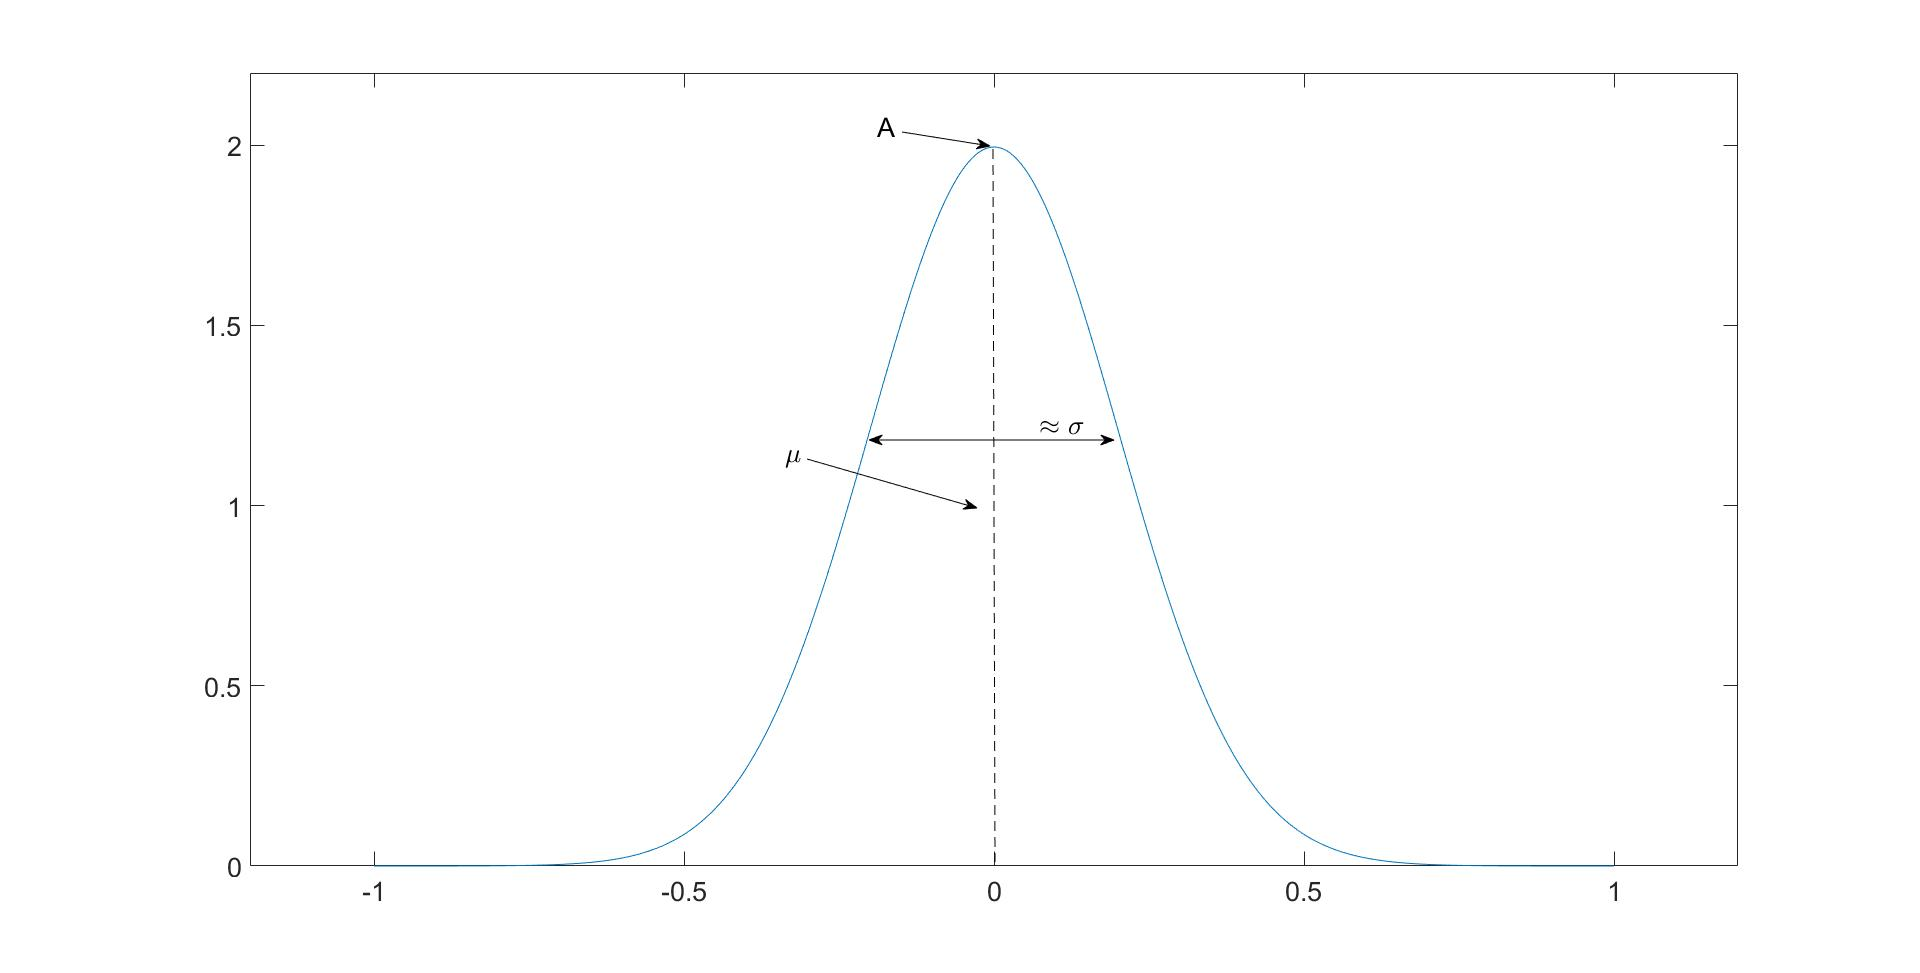
\includegraphics[width=0.95\textwidth]{gauss/bell_curve}
  \caption{One dimensional Gaussian Distribution, $\mu$=0, $\sigma$=0.2 and $A$ = 2}
  \label{fig:gauss}
\end{figure}

The Gaussian distribution may be expressed in more dimensions than one, as it has been expressed thus far. It may be useful to model the distribution in more than one dimension as data sets may be comprised entries of more than one dimension. For example a digital image is specified by two dimensions in the x and y direction. Equation \ref{eq:gauss_2D} describes the Circular Gaussian distribution function, circular meaning the standard deviation for both random variables is the same, for the independent random variables X and Y. Figure \ref{fig:gauss_2D} visualizes the two dimensional distribution, anything beyond 2D cannot be easily visualized. 

\begin{equation}
f(x,y) = \frac{1}{2\pi\sigma}e^\frac{{-\big[(x-\mu_x)^2 + (y-\mu_y)^2\big]}}{2\sigma^2}
\label{eq:gauss_2D}
\end{equation}

\begin{figure}[H]
  \centering
  \centering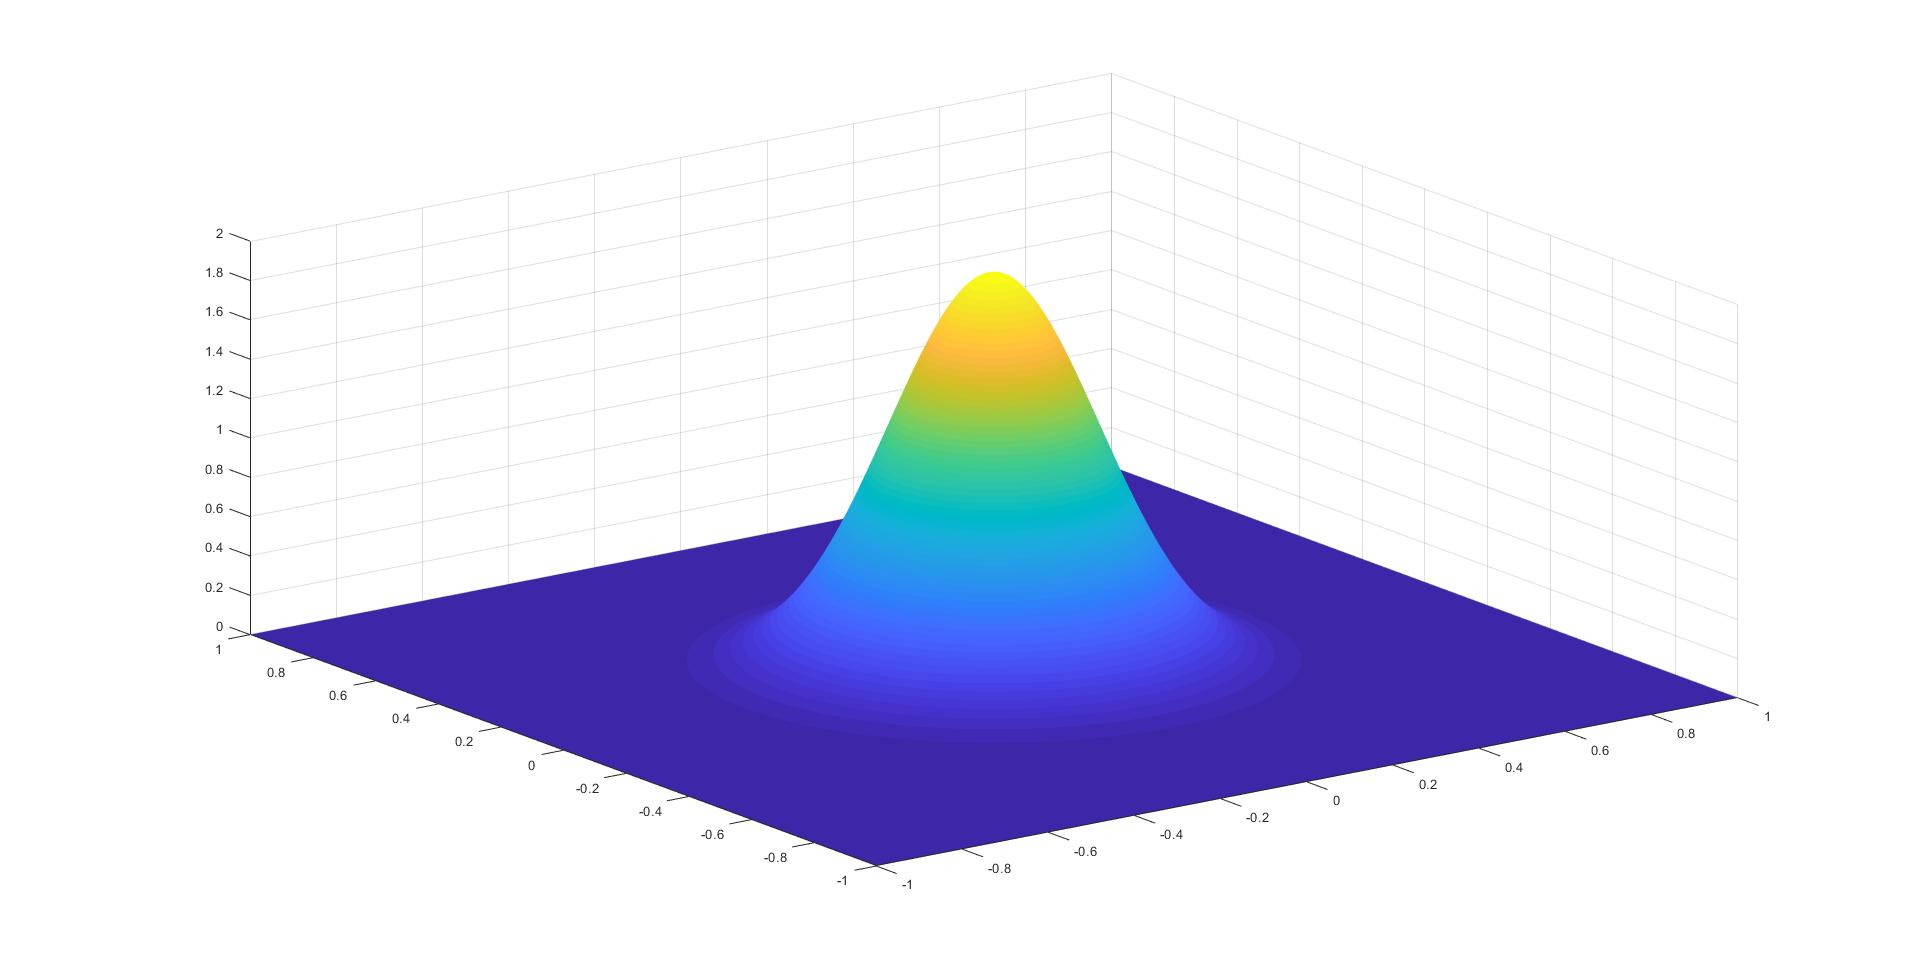
\includegraphics[width=0.9\textwidth]{gauss2D}
  \caption{The 2D Gaussian Distribution Function, $\mu_x$= 0, $\mu_y$= 0, $\sigma$= 0.2 and $A$ = 2.}
  \label{fig:gauss_2D}
\end{figure}







  
  
